%%%%%%%%%%%%%%%%%%%%%%%%%%%%%%%%%%%%%%%%%%%%%%%%%%%%%%%%%%%%%%%%%%%%%%%%%%%%%%%%
%2345678901234567890123456789012345678901234567890123456789012345678901234567890
%        1         2         3         4         5         6         7         8
% DOCUMENT CLASS
\documentclass[oneside,12pt]{Classes/RoboticsLaTeX}

% USEFUL PACKAGES
% Commonly-used packages are included by default.
% Refer to section "Book - Useful packages" in the class file "Classes/RoboticsLaTeX.cls" for the complete list.
\usepackage{amsmath}
\usepackage{amsfonts}
\usepackage{algorithm}
\usepackage{algorithmic}
\usepackage{geometry}
\usepackage{url}
\usepackage{hyperref}
\usepackage{graphicx} % Required for inserting images

% SPECIAL COMMANDS
% correct bad hyphenation
\hyphenation{op-tical net-works semi-conduc-tor}
%% ignore slightly overfull and underfull boxes
%\hbadness=10000
%\hfuzz=50pt
% declare commonly used operators
\DeclareMathOperator*{\argmax}{argmax}

% HEADER
\ifpdf
    \pdfinfo {/Title (Example of M.Sc. Thesis with RoboticsLaTeX template)
              /Creator (TeX)
              /Producer (pdfTeX)
              /Author (Fabio Guelfi)
              /CreationDate (D:20141024182500) %format D:YYYYMMDDhhmmss
              /ModDate (20141024182500)
              /Subject (Example of PhD Thesis with RoboticsLaTeX template)
              /Keywords (PhD, Thesis, Example, RoboticsLaTeX)}
    \pdfcatalog {/PageMode (/UseOutlines)
                 /OpenAction (fitbh) }
\fi




\title{Example of PhD Thesis with RoboticsLaTeX template}

\ifpdf
  \author{\myhlink{mailto:name@unige.it}{Fabio Guelfi}}
  \collegeordept{\myhlink{http://www.dibris.unige.it}{DIBRIS - Department of Computer Science, Bioengineering, Robotics and System Engineering}}
  \university{\myhlink{http://www.unige.it}{University of Genova}}
  \supervisors{
  	  \begin{tabular}{rl}
  		Prof. &  \myhlink{mailto:name@unige.it}{Name Surname} \\
  		Prof. & \myhlink{mailto:name@unige.it}{Name Surname}  \\
  	\end{tabular}
  	}
  \crest{
\includegraphics[width=50mm]{logo_unige}}
\else
  \author{Barbara Bruno, Fulvio Mastrogiovanni}
  \collegeordept{DIBRIS - Department of Computer Science, Bioengineering, Robotics and System Engineering}
  \university{University of Genova}
  \crest{
\includegraphics[width=50mm]{logo_unige}}
\fi



% DECLARATION
% Use the following command to change the declaration text:
%\renewcommand{\submittedtext}{INSERT NEW TEXT HERE}
\degree{Laurea Magistrale in Robotics Engineering}
\degreedate{February 31, 2015}

%%%%%%%%%%%%%%%%%%%%%%%%%%%%%%%%%%%%%%%%%%%%%%%%%%%%%%%%%%%%%%%%%%%%%%%%%%%%%%%%

\begin{document}

% A page with the abstract and running title and author etc may be
% required to be handed in separately. If this is not so, comment
% the following 3 lines:
% \begin{abstractseparate}
%   \section{Abstract}
Qui scrivere abstract finale andando a ricoprire tutto ciò che è stato cstruito per
la tesi\\
% \end{abstractseparate}

\maketitle

% add an empty page after title page
\newpage\null\thispagestyle{empty}\newpage

% set the number of sectioning levels that get number and appear in the contents
\setcounter{secnumdepth}{3}
\setcounter{tocdepth}{3}

\frontmatter
\begin{originality}

I, Fabio Guelfi, hereby declare that this thesis is my own work and all sources of information and ideas have been acknowledged appropriately. This work has not been submitted for any other degree or academic qualification. I understand that any act of plagiarism, reproduction, or use of the whole or any part of this thesis without proper acknowledgment may result in severe academic penalties.
\end{originality}
%%%%%%%%%%%%%%%%%%%%%%%%%%%%%%%%%%%%%%%%%%%%%%%%%%%%%%%%%%%%%%%%%%%%%%%%%%%%%%%%
%2345678901234567890123456789012345678901234567890123456789012345678901234567890
%        1         2         3         4         5         6         7         8
% THESIS ACKNOWLEDGEMENTS

% Use the following style if the acknowledgements are long:
%\begin{acknowledgementslong}
%\end{acknowledgmentslong}

\begin{acknowledgements}


This is an optional section, where you can write acknowledgments.
Don't forget to acknowledge your supervisor!


\end{acknowledgements}

%%%%%%%%%%%%%%%%%%%%%%%%%%%%%%%%%%%%%%%%%%%%%%%%%%%%%%%%%%%%%%%%%%%%%%%%%%%%%%%%
%2345678901234567890123456789012345678901234567890123456789012345678901234567890
%        1         2         3         4         5         6         7         8
% THESIS DEDICATION

\begin{dedication}

\begin{flushright}
This is a short, optional, dedication.
To all the Master and PhD students of Robotics Engineering at the University of Genova.
\end{flushright}

\end{dedication}

% ----------------------------------------------------------------------

%%% Local Variables: 
%%% mode: latex
%%% TeX-master: "../thesis"
%%% End: 

\section{Abstract}
Qui scrivere abstract finale andando a ricoprire tutto ciò che è stato cstruito per
la tesi\\

\tableofcontents
\listoffigures
%\printglossary  % Print the nomenclature (WAY TOO COMPLEX FOR ME NOW!)
%\addcontentsline{toc}{chapter}{Nomenclature}

\mainmatter
%%%%%%%%%%%%%%%%%%%%%%%%%%%%%%%%%%%%%%%%%%%%%%%%%%%%%%%%%%%%%%%%%%%%%%%%%%%%%%%%
%2345678901234567890123456789012345678901234567890123456789012345678901234567890
%        1         2         3         4         5         6         7         8
% THESIS CHAPTER

\chapter{Introduction}
\label{chap:first}
\ifpdf
    \graphicspath{{Chapter1/Figures/PNG/}{Chapter1/Figures/PDF/}{Chapter1/Figures/}{Chapter1/Figures/EPS/}}
\else
    \graphicspath{{Chapter1/Figures/EPS/}{Chapter1/Figures/}}
\fi


\section{Content}
In the introduction, please state clearly the context your work is framed within, and the motivations of your work. Furthermore, it is important to clarify your contribution (and not those of the group you work in - it is still an exam after all). Provide an outline of the thesis.


\section{Basic commands}
\label{sec:basic_commands}
This is a citation: \cite{cacciaActiveSonarbasedBottomfollowing1999}. Make sure to correctly enter all the bibliographic details. It is important that you double check them when retrieving the bibtex file from a source such as Google Scholar. Consistency in the references is valued by the Committee.

This is an emphasized word: \emph{global}.

This is a reference to another part of the thesis: Chapter \ref{chap:introduction}.

This is an enumerated list:
\begin{enumerate}
\item first item.
\item second item.
\end{enumerate}

This is an in-line equation: $x-$.

This is a word in quotes: ``regular''.

\section{Equation}
\label{sec:equation}

This is an equation:
\begin{equation}
{\mathcal{U}}_k(s_k) = \frac{P_k}{C_k}.
\label{eq:normal}
\end{equation}

Equations follow the punctuation rules, as if they were inline with the text.

This is an equation split over multiple lines:
\begin{equation}\label{eq:Split}
\begin{aligned}
x_{k}&={\mathcal{F}}(x_{k-1},u_{k},w_{k-1}),\\
z_{k}&={\mathcal{H}}(x_{k},v_{k}).
\end{aligned}
\end{equation}

This is an example of equation with matrices:
\begin{equation}
\mathcal{Q}_l  = \frac{{d_l ^2 \sigma _\phi  ^2 }}{2} {\begin{bmatrix}
   {2\sin ^2 \phi _l } & { - \sin 2\phi _l }  \\
   { - \sin 2\phi _l } & {2\cos ^2 \phi _l }  \\
\end{bmatrix}}
 \begin{bmatrix}{cc}
   {\frac{{\sigma _d ^2 }}{2} {\begin{array}{cc}
   {2\cos ^2 \phi _l } & {\sin 2\phi _l }  \\
   {\sin 2\phi _l } & {2\sin ^2 \phi _l }  \\
\end{array}}}  \\
\end{bmatrix}. \\
\label{eq:defQ}
\end{equation}

This is a reference to the Equation \ref{eq:Split}. Avoid using unnumbered equations as it makes it difficult to reference them during a discussion. Also, be consistent in the use of matrix or vector notation. For example, $\dot{\vec{x}}= \mat{A}\vec{x} + \mat{B}\vec{u}$ or $\vec{y} = \alpha \vec{x}$, where the $\alpha$ is a scalar. You can change the corresponding definitions in the class file, as long as you remain consistent.

\section{Figure}
\label{sec:figure}

I add a figure.
\begin{figure}[H]
\centering
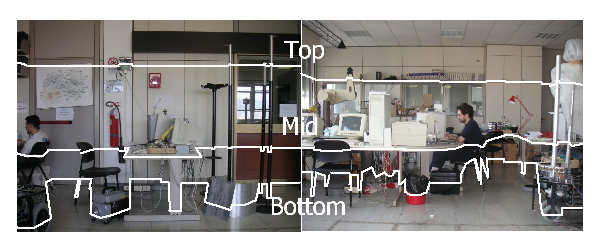
\includegraphics[width=5.0in]{Views}
\caption{Scan profiles: \emph{bottom}, \emph{mid} and \emph{top view}.}
\label{fig:views}
\end{figure}
Make sure that figures axis are readable. Make sure to label all the units on both axes. The width of the lines should be also crosschecked for readability (the typical MATLAB plot might need higher line width). Double check that legends are present. Figures' captions should allow the reader to fully understand the figure.

This is a reference to Figure \ref{fig:views}.

\section{Table}
The suggested packages for tables is tabular. There are many examples on the Internet. In general, avoid vertical lines, and use horizontal lines sparingly. Here S allows to align to the decimal point.
 
\begin{tabular}{SSSSSSSS} \toprule
	{$m$} & {$\Re\{\underline{\mathfrak{X}}(m)\}$} & {$-\Im\{\underline{\mathfrak{X}}(m)\}$} & {$\mathfrak{X}(m)$} & {$\frac{\mathfrak{X}(m)}{23}$} & {$A_m$} & {$\varphi(m)\ /\ ^{\circ}$} & {$\varphi_m\ /\ ^{\circ}$} \\ \midrule
	1  & 16.128 & +8.872 & 16.128 & 1.402 & 1.373 & -146.6 & -137.6 \\
	2  & 3.442  & -2.509 & 3.442  & 0.299 & 0.343 & 133.2  & 152.4  \\
	3  & 1.826  & -0.363 & 1.826  & 0.159 & 0.119 & 168.5  & -161.1 \\
	4  & 0.993  & -0.429 & 0.993  & 0.086 & 0.08  & 25.6   & 90     \\ \midrule
	5  & 1.29   & +0.099 & 1.29   & 0.112 & 0.097 & -175.6 & -114.7 \\
	6  & 0.483  & -0.183 & 0.483  & 0.042 & 0.063 & 22.3   & 122.5  \\
	7  & 0.766  & -0.475 & 0.766  & 0.067 & 0.039 & 141.6  & -122   \\
	8  & 0.624  & +0.365 & 0.624  & 0.054 & 0.04  & -35.7  & 90     \\ \midrule
	9  & 0.641  & -0.466 & 0.641  & 0.056 & 0.045 & 133.3  & -106.3 \\
	10 & 0.45   & +0.421 & 0.45   & 0.039 & 0.034 & -69.4  & 110.9  \\
	11 & 0.598  & -0.597 & 0.598  & 0.052 & 0.025 & 92.3   & -109.3 \\ \bottomrule
\end{tabular}
\section{Algorithm} 
\label{sec:algorithm}

This is an algorithm:
\begin{algorithm}
\label{alg:SMS}
\caption{Split \& Merge [\& Split]}
\begin{algorithmic} [1]
\REQUIRE{A scan $s$. A stack $\mathcal{L}$. A counter $j$. A threshold $\tau$}
\ENSURE{$\lambda \leftarrow \mathcal{M}(s)$, $j=1, ..., |\lambda|$}
\STATE{$\mathcal{L}$ = \texttt{push}($s$)}
\STATE{$j \leftarrow 1$}
\WHILE{$\mathcal{L}$ $\neq$ $\varnothing$}
\STATE{$\mathcal{L}$ = \texttt{pop}($s_{top}$)}
\STATE{$l_j$ $\leftarrow$ \texttt{fitting}($s_{top}$)}
\STATE{$q_k = \argmax_{q}\texttt{dist(l$_j$,q)}$}
\IF{$\texttt{dist(l$_j$,$q_k$)} < \tau$}
\STATE{$j \leftarrow j+1$}
\STATE{\texttt{continue}}
\ELSE
\STATE{$s_a \leftarrow$ \texttt{sub}($s_{top}$, 1, $k$)}
\STATE{$s_b \leftarrow$ \texttt{sub}($s_{top}$, $k+1$, $|s|$)}
\STATE{$\mathcal{L}$ = \texttt{push}($s_a$)}
\STATE{$\mathcal{L}$ = \texttt{push}($s_b$)}
\ENDIF
\ENDWHILE
\STATE{\{$l_j$\} $\leftarrow$ \texttt{merge}(\{$l_j$\})}
\STATE{\{$l_j$\} $\leftarrow$ \texttt{split}(\{$l_j$\})}
\end{algorithmic}
\end{algorithm}

% NOMI DA RIDEFINIRE

\section{Historical background}
\subsection{Marine robotics}
\subsection{Autonomous navigation}
\subsection{Underwater mission in seabed inspection}

\section{Problem statement}
\section{Motivation}

\section{Previous work and main contribution}
\subsection{Motion control of vehicles}
\subsection{Terrain following types} 
\subsection{EKF and echosonar usage}
\subsection{Caccia PAPER AND SIMILAR}

\section{Thesis outline}
%%%%%%%%%%%%%%%%%%%%%%%%%%%%%%%%%%%%%%%%%%%%%%%%%%%%%%%%%%%%%%%%%%%%%%%%%%%%%%%%
%2345678901234567890123456789012345678901234567890123456789012345678901234567890
%        1         2         3         4         5         6         7         8
% THESIS CONCLUSIONS
\def\baselinestretch{1}
\chapter{Conclusions}
\label{chap:conclusions}
\ifpdf
    \graphicspath{{Conclusions/Figures/PNG/}{Conclusions/Figures/PDF/}{Conclusions/Figures/}}
\else
    \graphicspath{{Conclusions/Figures/EPS/}{Conclusions/Figures/}}
\fi
\def\baselinestretch{1.66}

Write the conclusions here...
% Concentrarsi su:
% 1) Riepilogo dei risultati ottenuti
% 2) Implicazioni per la comunità scientifica e per l'industria
% 3) Trovare vantaggi e svantaggi del metodo per l'industria (es: Mappatura batimetrica di precisione, 
% Ispezione e manutenzione subacquea, Monitoraggio ambientale, Ricerca oceanografica e archeologia subacquea)
% 4) Limitazioni dello studio
% 5) Prospettive future e direzioni di ricerca

% Questo approccio non solo migliora le prestazioni operative di un AUV, ma apre la strada a missioni più lunghe, 
% sicure ed efficienti, con un impatto significativo in applicazioni scientifiche, industriali e ambientali.

\appendix
%%%%%%%%%%%%%%%%%%%%%%%%%%%%%%%%%%%%%%%%%%%%%%%%%%%%%%%%%%%%%%%%%%%%%%%%%%%%%%%%
%2345678901234567890123456789012345678901234567890123456789012345678901234567890
%        1         2         3         4         5         6         7         8
% THESIS APPENDIX

\chapter{Extra}
\label{chap:appendixA}

Write here...

\bibliographystyle{Classes/RoboticsBiblio}    % bibliography style
\renewcommand{\bibname}{References}           % change default name Bibliography to References
\bibliography{references}          % References file
\addcontentsline{toc}{chapter}{References}    % add References to contents page

\end{document}
